\chapter{Theory and motivations}
\label{CHAPTER:TheoryAndMotivations}

\glsresetall % Resetting all acronyms

% STATUS: DONE

The goal of particle physics is to study the most fundamental constituents of matter and understand how they interact with each other. The \gls{SM} of particle physics will briefly introduced and the Higgs mechanism explained and the search for Higgs boson decaying invisibly decays will be motivated. Throughout this chapter Einstein summation convention, Feynman slash notation and natural units are used, where $\hbar=c=1$. Additionally, greek letters are used to label the four vectors, and gauge group generators use roman letters.

%%%%%%%%%%%%%%%%%%%%%%%%%%%%%%%%%%%%%%%%%%%%%%%%%%%%%%%%%%%%%%%%%%%%%%%%%%%%%%%%%%%%%%%
%%% SECTION
%%%%%%%%%%%%%%%%%%%%%%%%%%%%%%%%%%%%%%%%%%%%%%%%%%%%%%%%%%%%%%%%%%%%%%%%%%%%%%%%%%%%%%%
\section{Standard Model of Particle Physics}

% STATUS: DONE

The \gls{SM} of particle physics is a \gls{QFT} including both relativistic and quantum mechanical effects. It describes the electromagnetic, weak nuclear and strong forces and their interaction with matter. This theory is one of the most successful theories ever made and was able to describe data from a wide range of experimental measurements. Before its discovery in 2012 \cite{ARTICLE:ATLAS_HiggsDiscovery,ARTICLE:CMS_HiggsDiscovery} the Higgs boson was the only missing particle that was predicted by this theory and not yet found. 

Although its success, the \gls{SM} does not explain some phenomena observed in nature, like the presence of large quantity of \textit{dark matter} in the universe, or the even more mysterious \textit{dark energy}. The discovery of the Higgs boson could allow to probe the production of dark matter directly, through its decay into these elusive particles. 

%%%%%%%%%%%%%%%%%%%%%%%%%%%%%%%%%%%%%%%%%%%%%%%%%%%%%%%%%%%%%%%%%%%%%%%%%%%%%%%%%%%%%%%
%%% SUBSECTION
%%%%%%%%%%%%%%%%%%%%%%%%%%%%%%%%%%%%%%%%%%%%%%%%%%%%%%%%%%%%%%%%%%%%%%%%%%%%%%%%%%%%%%%
\subsection{Fundamental matter particles}
\label{SUBSECTION:Theory_SM_ParticlesAndForces}

% STATUS: DONE 

All particles of matter considered fundamental observed until now are spin-$\frac{1}{2}$ fermions. The equations of motion for a spin-$\frac{1}{2}$ dirac fermion with a mass $m$ can be found in equation \ref{EQUATION:Theory_SM_ParticlesAndForces_Dirac}.

\begin{equation}
(i\gamma^{\mu}\partial_{\mu} - m)\psi = 0
\label{EQUATION:Theory_SM_ParticlesAndForces_Dirac}
\end{equation}

In this equation the matrices $\gamma^{\mu}$, $\mu\in{0,1,2,3}$, are defined by the anti-commutator relation $\gamma^{\mu}\gamma^{\nu}+\gamma^{\mu}\gamma^{\nu} = 2\eta^{\mu\nu}I_{4}$ where $\eta^{\mu\nu}$ is the flat space-time metric $(+,-,-,-)$ and $I_{4}$ is the $4\times4$ identity matrix. The solutions for the Dirac fermion equation of motion, $\psi$, are the massive particle and anti-particle states, with momentum $\mathbf{p}$ and energy $E$, which satisfy the relativistic expression, $E^{2} = \mathbf{p}\cdot\mathbf{p} + m^{2}$.

Fundamental fermions can be split in two categories depending if they interact (quarks) or not (leptons) with the strong nuclear force. Both this categories of particles can grouped into three generations, with similar properties between them but increasing mass. While lepton can be examined isolated, free quarks are not observed in nature, they are confined in composed structures of three (baryons) or two (mesons) quarks. Table \ref {TABLE:Theory_SM_ParticlesAndForces_MatterParticle} shows a summary of the know fundamental.

\begin{table}[!htb]
\centering
\begin{tabular}{|c||c|c|c||c|c|c|}
\hline
 & \multicolumn{3}{c||}{Leptons (J=1/2)} & \multicolumn{3}{c|}{Quarks (J=1/2)} \\
\hline
Generation                &     Symbol &            Mass & Q/e & Symbol &           Mass & Q/e \\
\hline\hline
\multirow{2}{*}{$1^{st}$} & e          &     $511\,\keV$ &   1 &      u &    $2.3\,\MeV$ &  2/3 \\
                          & $\nu_e$    &     $< 2\, \eV$ &   0 &      d &    $4.8\,\MeV$ & -1/3 \\
\hline
\hline
\multirow{2}{*}{$2^{nd}$} & $\mu$      &  $   106\,\MeV$ &   1 &      c &  $1.275\,\GeV$ &  2/3 \\
                          & $\nu_\mu$  &  $< 0.19\,\MeV$ &   0 &      s &     $95\,\MeV$ & -1/3 \\
\hline
\hline
\multirow{2}{*}{$3^{rd}$} & $\tau$     & $   1777\,\MeV$ &   1 &      t & $173.21\,\GeV$ &  2/3 \\
                          & $\nu_\tau$ & $< 18.2 \,\MeV$ &   0 &      b &   $4.66\,\GeV$ & -1/3 \\
\hline
\end{tabular}
\caption[List of leptons and their fundamental properties]{List of fermions grouped in generations and split in fermions and quarks and their fundamental properties \cite{ARTICLE:PDG2014}.}
\label{TABLE:Theory_SM_ParticlesAndForces_MatterParticle}
\end{table}

\subsection{Fundamental forces}

Gauge bosons mediate the fundamental forces of nature. All observed force mediators up to now are spin-1, which arises from symmetry considerations which the relevant theory possesses. The \gls{QFT} that describes the electromagnetism is \gls{QED} 
% TODO: Continue

\begin{table}[!htb]
  \centering
  \begin{tabular}{|c|c|c|c|c|}
  \hline
  \multicolumn{4}{|c|}{Bosons} \\
  \hline
   Particle Name & Mass ($GeV$) &     Q/e & Spin \\
  \hline
  \hline
  Photon ($\gamma$) &                  0 &       0 &    1 \\
  \hline
  $W^\pm$           & $80.385 \pm 0.015$ & $\mp 1$ &    1 \\
  $Z^0$             & $91.1876\pm0.0021$ &       0 &    1 \\
  \hline
  Gloun (g)         &                  0 &       0 &    1 \\
  \hline
  \end{tabular}
  \caption[List of bosons and their fundamental properties]{List of force carrying bosons and their fundamental properties \cite{ARTICLE:PDG2014}.}
  \label{TABLE:Theory_SM_ParticlesAndForces_BosonProperties}
\end{table}


% The fundamental forces of nature are mediated by the exchange of gauge bosons. They are all spin-1 particles which arise from consideration of the symmetries which the relevant theory possesses (See Section~\ref{sec:ewksymmetry}). The quantum field theories of electromagnetism, Quantum Electro-dynamics (QED), and the strong nuclear force, Quantum Chromo-dynamics (QCD), yield massless mediator bosons, the photon and the gluons, which are a direct consequence of the gauge invariance of those theories. Despite this, the typical ranges over which the two interactions occur are dramatically different; strong interaction effects are only apparent on a scale of around $10^{-15}$m whereas the range of electromagnetic interactions are effectively infinite.
% 
% The mediators of the weak nuclear and electromagnetic forces arise through the unification of the theories of weak and electromagnetic interactions and the mixing of the associated gauge fields. The weak gauge bosons, $W^{\pm}$ and $Z$, unlike the photon and gluons, have a finite mass which has been measured experimentally~\citep{combinedWmass,pdg}. A summary of the fundamental gauge bosons of the Standard Model is given in Table~\ref{tab:bosons}. A quantum description of gravity is not included in the Standard Model. This is a reasonable approximation as the strength of this interaction is much smaller than the other three, thereby having no impact on the predictive power of the model.
% 
% \begin{table}[htbp!]
% \begin{tabular}{|l|l c|c|c|}
% \hline 
%         & \textbf{Mediator Particle} & & \textbf{Charge} & \textbf{Mass (GeV)} \\
% \hline
% Electromagnetism & photon & $\gamma$                    & 0 & 0   \\
% \hline
% Strong Nuclear   & gluon  & $g_{j},$ $j\in\left\{1,\cdots8\right\}$     & 0 & 0   \\
% \hline
% Weak Nuclear     &  &  $W^{+}$ & +1 & 80.39 \\
%                  &  &  $W^{-}$ & -1 & 80.39 \\
%                  &  &  $Z$     & 0  & 91.19 \\
% \hline
% \end{tabular}
% \caption{Fundamental gauge bosons in the Standard Model. All of the gauge-bosons are spin-1 particles. The masses of the $W^{\pm}$ and $Z$ bosons are taken from References~\citep{combinedWmass} and~\citep{pdg} respectively.}
% \label{tab:bosons}
% \end{table}

\subsection{Electroweak Gauge Symmetry}

% \subsection{Electroweak Gauge Symmetry}
% \label{sec:ewksymmetry}
% 
% Symmetries in nature are often found to relate to some underlying physical principle or fundamental law. It was first shown by Emmy Noether that for any physical system which can be described in the Lagrangian formalism, any symmetry of the Lagrangian has an associated conserved quantity~\cite{noether}. In the context of dynamical quantum theories, the particular characteristics of particle interactions can be used to constrain the appropriate Lagrangian by identifying a particular group of transformations under which the Lagrangian should be symmetric (invariant). 
% 
% One of the major achievements of the twentieth century in the development of the Standard Model was the unification of the electromagnetic and weak interactions~\citep{glashow,weinberg,salam}. The original proposal, by Glashow in 1961, was to construct a theory which incorporates the characteristics of the weak and electromagnetic interactions by associating them with a particular symmetry group~\citep{glashow}. The physical nature of electroweak interactions is encoded into a Lagrangian which is invariant under transformations of the group $\sutwol\times\uone$. This group has three generators for $\sutwol$, $T_{i} = \frac{1}{2}\tau_{i}$ where $\tau_{i},~i\in \{1,2,3 \}$ are the $2\times2$ Pauli-spin matrices, and one additional generator for $\uone$, $Y$. The quantum numbers associated with the $\sutwol$ group, weak isospin $t_{1,2,3}$, and $\uone$ group, hypercharge $y$, are related to the electric charge $Q$ as,
% 
% \begin{equation}
% Q = t_{3}+\frac{y}{2},
% \end{equation} 
% 
% where the factor of $\frac{\displaystyle 1}{\displaystyle 2}$ is chosen by convention. The associated gauge fields are $\hat{\mathbf{W}}_{\mu} = \left(\hat{W}_{\mu}^{1},\hat{W}_{\mu}^{2},\hat{W}_{\mu}^{3}\right)$ and $\hat{B}_{\mu}$. An example Lagrangian for interactions within the first leptonic generation of fermions, $\lagr_{G}$, is given in Equation~\ref{eqn:ewklagrangianeg},
% 
% \begin{eqnarray}
% \lagr_{G} & =& \bar{\chi}_{L}\gamma^{\mu}\left[i\partial_{\mu} 
%                    - g\frac{1}{2}\boldsymbol{\tau}\cdot\hat{\mathbf{W}_{\mu}}
%                    - g^{\prime}\left(-\frac{1}{2}\right)\hat{B}_{\mu}\right] \chi_{L}
% \nonumber \\
% & &                + \bar{e}_{R}\gamma^{\mu}\left[i\partial_{\mu} 
%                    - g^{\prime}(-1)\hat{B}_{\mu}\right]{e}_{R}
%                      -\frac{1}{4}
%                      \hat{\mathbf{W}}_{\mu\nu}\cdot\hat{\mathbf{W}}^{\mu\nu} 
%                      -\frac{1}{4}
%                      \hat{B}_{\mu\nu}\hat{B}^{\mu\nu}
% \label{eqn:ewklagrangianeg}
% \end{eqnarray}
% 
% where the bar notation denotes the adjoint of the field, $\bar{\psi}=\psi^{\dagger}\gamma^{0}$ and $\chi_{L}$ is the left handed component of the leptonic fermion doublet. The field tensors, $\hat{\mathbf{W}}_{\mu\nu}$ and $\hat{B}_{\mu\nu}$ given in Equations~\ref{eqn:wmunu} and~\ref{eqn:bmunu}, describe the kinematics of the gauge fields.
% 
% \begin{equation}
% \hat{\mathbf{W}}_{\mu\nu} = \partial_{\mu}\hat{\mathbf{W}}_{\nu} - \partial_{\nu}\hat{\mathbf{W}}_{\mu} - g \hat{\mathbf{W}}_{\mu}\wedge\hat{\mathbf{W}}_{\nu}
% \label{eqn:wmunu}
% \end{equation}
% \begin{equation}
% \hat{B}_{\mu\nu} = \partial_{\mu}\hat{B}_{\nu} - \partial_{\nu}\hat{B}_{\mu}.
% \label{eqn:bmunu}
% \end{equation}
% 
% Experimentally, it has been verified that the weak nuclear force explicitly violates parity, that is transformations under spatial inversions $x\rightarrow -x$~\citep{wu}. A fermionic field, $\psi$, can be projected into its left and right handed components, $\psi_{L}$ and $\psi_{R}$, using the operators $\frac{1}{2}(1\mp\gamma^{5})$ respectively, where $\gamma^{5} = \gamma^{0}\gamma^{1}\gamma^{2}\gamma^{3}$. As the weak nuclear force only interacts with left-handed fermions, right-handed components of the fermion fields are invariant under $\sutwol$ transformations. The right-handed component of the neutrino field therefore does not appear in the Lagrangian, $\lagr_{G}$, since it interacts with neither the electromagnetic nor the weak interactions. Under the $\sutwol\times\uone$ group, the left handed components of the leptonic fermion fields, $\chi_{L}$ of Equation~\ref{eqn:ewklagrangianeg}, transform as a doublet
% 
% \begin{equation}
% \chi_{L}  =   
% \everymath{\displaystyle} \begin{pmatrix}
% \nu_{e} \\ 
% e
% \end{pmatrix}_{L}
%  \longrightarrow 
% \exp(-i\boldsymbol\alpha\cdot\frac{\boldsymbol\tau}{2} - i\alpha) 
% \begin{pmatrix}
% \nu_{e} \\ 
% e
% \end{pmatrix}_{L}
% \end{equation}
% \label{eqn:doublettrans}
% whereas the right-handed component of the electron field transforms as a singlet.  
% \begin{equation}
% e_{R}
%  \longrightarrow 
% \exp(-2i{\alpha}) 
% e_{R}.
% \end{equation}
% 
% The transformations are ``local'' in the sense that the coefficients $\boldsymbol{\alpha}$ and $\alpha$ are functions of space-time. To maintain the symmetry under local transformations of this type, the gauge fields transform as follows, 
% 
% \begin{eqnarray}
% \hat{\mathbf{W}}_{\mu} & 
%  \longrightarrow & 
% \hat{\mathbf{W}}_{\mu} - \frac{1}{g}\partial_{\mu}\boldsymbol{\alpha} 
%         - \boldsymbol{\alpha}\wedge\hat{\mathbf{W}}_{\mu} \\
% \hat{{B}}_{\mu} & 
%  \longrightarrow & 
% \hat{{B}}_{\mu} - \frac{1}{g^{\prime}}\partial_{\mu}{\alpha} 
% \end{eqnarray}
% 
% The Lagrangian of Equation~\ref{eqn:ewklagrangianeg} contains no explicit terms which relate to the mass of the electron ($m_{e}$). Including the electron's mass directly would require the addition of the term,
% 
% \begin{eqnarray}
% -m_{e}\bar{e}e  &=& -m_{e}\bar{e}\left[\frac{1}{2}\left(1-\gamma^{5}\right) 
%                     + \frac{1}{2}\left(1+\gamma^{5}\right)\right]e \nonumber \\
%                 &=& -m_{e}\left(\bar{e}_{R}e_{L} + \bar{e}_{L}e_{R}\right).
% \end{eqnarray}
% 
% As $e_{L}$ transforms as a member of a doublet and $e_{R}$ as a singlet, the addition of this term to Equation~\ref{eqn:ewklagrangianeg} would break the symmetry of the Lagrangian which motivated its construction, namely transformations under the $\sutwol$ group~\citep{aitchison}.
% 
% The physical electroweak boson fields, $\hat{W}_{\mu}^{\pm}$, $\hat{Z}_{\mu}$ and photon field, $\hat{A}_{\mu}$, are obtained through a mixture of the electroweak gauge fields as,
 
\begin{eqnarray}
\hat{W}_{\mu}^{\pm} & = &  \sqrt{\frac{1}{2}} \left( \hat{W}_{\mu}^{1} \mp i \hat{W}_{\mu}^{2} \right) \nonumber \\
\hat{Z}_{\mu} &  = & \cos\theta_{w} \hat{W}_{\mu}^{3} - \sin\theta_{w} \hat{B}_{\mu} \nonumber \\
\hat{A}_{\mu} &  = & \sin\theta_{w} \hat{W}_{\mu}^{3} + \cos\theta_{w} \hat{B}_{\mu},
\label{eqn:ewkbosons}
\end{eqnarray}
 
% where the mixing angle, $\theta_{w} = \tan^{-1}{\frac{g^{\prime}}{g}}$, relates the couplings of the weak neutral and electromagnetic interactions. As expected, there is no term which corresponds to the mass of the photon, however, the same is true for the $W$ and $Z$ bosons. The masses of the $W$ and $Z$ bosons, given in Table~\ref{tab:bosons}, have been measured experimentally and found to be non-zero. The inclusion of mass terms for these bosons in Equation~\ref{eqn:ewklagrangianeg} would also break the symmetry of the Lagrangian. Furthermore, it has been shown that the inclusion of these mass terms results in a loss of re-normalizability of the theory, making it less powerful for predicting observables such as cross-sections and decay rates~\citep{halzen}. Instead, these masses can be generated via a spontaneous, rather than explicit, breaking of the symmetry.

\subsection{Spontaneous Symmetry Breaking: The Higgs Mechanism}

% \subsection{Spontaneous Symmetry Breaking: The Higgs Mechanism}
% 
% In quantum field theory, a symmetry is ``spontaneously'' broken when the Lagrangian itself remains invariant while the vacuum state, for which the Hamiltonian of the theory attains its minimum, does not~\cite{aitchison}. In the context of the electroweak theory, spontaneous symmetry breaking is achieved through the introduction of a complex scalar field which attains a non-zero vacuum expectation value (VEV)~\citep{Higgs:1964ia,PhysRev.155.1554,Higgs:1964pj,Guralnik:1964eu,PhysRev.145.1156}. This field is an $SU(2)$ doublet,
 
\begin{equation}
\phi = 
\everymath{\displaystyle} \begin{pmatrix}
\phi^{+} \\ 
\phi^{0}
\end{pmatrix}
\end{equation}

% The Lagrangian, $\lagr_{G}$, of Equation~\ref{eqn:ewklagrangianeg} is modified to include
% an additional term which is $\sutwol\times\uone$ invariant, $\lagr_{\phi}$
% given by, 

% \begin{equation}
% \lagr_{\phi}=(\hat{D}_{\mu}\phi)^{\dagger}(\hat{D}^{\mu}\phi)  
%             +\mu^{2} \phi^{\dagger}\phi - \frac{\lambda}{4}(\phi^{\dagger}\phi)^{2},
% \label{eqn:higgslagr}
% \end{equation}
%
%where the covariant derivative $\hat{D}^{\mu}$ which acts on $\phi$ is given by,
%
% \begin{equation}
% \hat{D}^{\mu} = \partial^{\mu} + ig\frac{1}{2}\boldsymbol{\tau}\cdot\hat{\mathbf{W}}^{\mu}
%                 + ig^{\prime}\frac{1}{2} \hat{B}^{\mu}.
% \end{equation}
% 
% The second two terms in Equation~\ref{eqn:higgslagr} correspond to the Higgs potential. In order to generate masses for the gauge bosons, the parameters, $\mu$ and $\lambda$, must satisfy $\mu^{2}>0$ and $\lambda>0$. The choice of non-zero VEV must then be made so that only the $W$ and $Z$ bosons acquire mass, while the symmetry associated with electromagnetism remains unbroken, leaving the photon massless. The choice suggested by Weinberg in 1967~\citep{weinberg} was,
% 
% \begin{equation}
% \mathrm{VEV} = \langle0|\phi|0\rangle = 
% \everymath{\displaystyle} \begin{pmatrix}
% 0 \\ 
% \frac{v}{\sqrt{2}}
% \end{pmatrix},
% \end{equation}
% 
% where $v= \frac{\displaystyle 2\mu}{\displaystyle \sqrt{\lambda}}$. In order to obtain the physical particle spectrum, perturbations around the vacuum state are considered. If $\boldsymbol{\hat{\theta}}$ and $\hat{H}$ represent small variations in the four degrees of freedom of the field $\phi$ then, 
% 
% \begin{equation}
% \phi = \exp(-i\boldsymbol{\hat{\theta}}\cdot\frac{1}{2v}\boldsymbol{\tau}) 
% \everymath{\displaystyle} \begin{pmatrix}
% 0 \\ 
% \frac{1}{\sqrt{2}}(v+\hat{H})
% \end{pmatrix}.
% \end{equation}
% 
% This can be simplified by choosing the phase fields $\boldsymbol{\hat{\theta}}$ to be zero. The Lagrangian obtained by inserting $\phi$ with this form into Equation~\ref{eqn:higgslagr} and adding it to the Lagrangian of Equation~\ref{eqn:ewklagrangianeg} is,
% 
% \begin{eqnarray}
% \lagr_{\phi}+\lagr_{G} 
%              & = &   \frac{1}{2} \partial_{\mu} \hat{H} \partial^{\mu} \hat{H} 
%              - \mu^{2} \hat{H}^{2} 
%              + \frac{1}{8} g^{2}v^{2}\hat{W}_{1\mu}\hat{W}_{1}^{\mu}
%              + \frac{1}{8} g^{2}v^{2}\hat{W}_{2\mu}\hat{W}_{2}^{\mu}    
% \nonumber \\
%             & & - \frac{v^{2}}{8} \left(g^{2}+{g^{\prime}}^{2}\right)\hat{Z}_{\mu}\hat{Z}^{\mu}
%              + KB ,
% \label{eqn:lagrssb}
% \end{eqnarray}
% 
% where only terms which are at most second order in the fields are kept, illustrating the physical particle spectrum, and the fermion fields are dropped altogether. The relation between the $\hat{W}^{\mu}_{3}$ and $\hat{B}^{\mu}$ fields from Equation~\ref{eqn:ewkbosons} has been used to obtain the physical photon, $\hat{A}^{\mu}$, and $\hat{Z}^{\mu}$ fields. From this form of the Lagrangian, it is clear that the $\hat{W}_{1}^{\mu}$, $\hat{W}^{\mu}_{2}$ and $\hat{Z}$ fields acquire mass. As the $\hat{W}_{1}^{\mu}$ and $\hat{W}^{\mu}_{2}$ fields mix to form the physical $\hat{W}^{\pm}$ fields, the $W^{\pm}$ bosons acquire a mass of $m_{W} = \frac{\displaystyle gv}{\displaystyle 2}$. The mass of the $Z$ boson is given by $m_{Z}=\frac{\displaystyle v}{\displaystyle 2}\sqrt{g^{2}+{g^{\prime}}^{2}}$, while there is no term associated with the mass of the photon. An additional scalar field, $\hat{H}$ (the Higgs boson), remains in the Lagrangian with mass $\sqrt{2}\mu$. The term $KB$ in Equation~\ref{eqn:lagrssb} denotes additional kinetic terms for the $\hat{W}^{\mu}_{1}$, $\hat{W}^{\mu}_{2}$, $\hat{Z}^{\mu}$ and $\hat{A^{\mu}}$ fields. The masses of the fermions are generated by adding Yukawa coupling terms,
% 
% \begin{equation} 
% -\lambda_{f} \bar{\chi}_{L} \phi \psi_{R} + \lambda_{f^{\prime}}\bar{\psi}_{R}(-i\tau_{2}\phi^{*})\chi_{L},
% \end{equation}
% 
% to $\lagr_{\phi}$. The couplings $\lambda_{f}$, $f=u,d,e,\mu\cdots$,  are directly related to the mass of the fermions, specifically $\lambda_{f}\propto m_{f}$ such that the heavier fermions have stronger coupling to the Higgs boson. Although the SM does not predict the values of these couplings, the masses of the fermions are experimentally measurable allowing access to, and providing constraints on, the properties of the Higgs boson.
% 

%%%%%%%%%%%%%%%%%%%%%%%%%%%%%%%%%%%%%%%%%%%%%%%%%%%%%%%%%%%%%%%%%%%%%%%%%%%%%%%%%%%%%%%
%%% SUBSECTION
%%%%%%%%%%%%%%%%%%%%%%%%%%%%%%%%%%%%%%%%%%%%%%%%%%%%%%%%%%%%%%%%%%%%%%%%%%%%%%%%%%%%%%%
\subsection{Searching for the SM Higgs boson}


\begin{figure}[htbp]
\subfloat[]{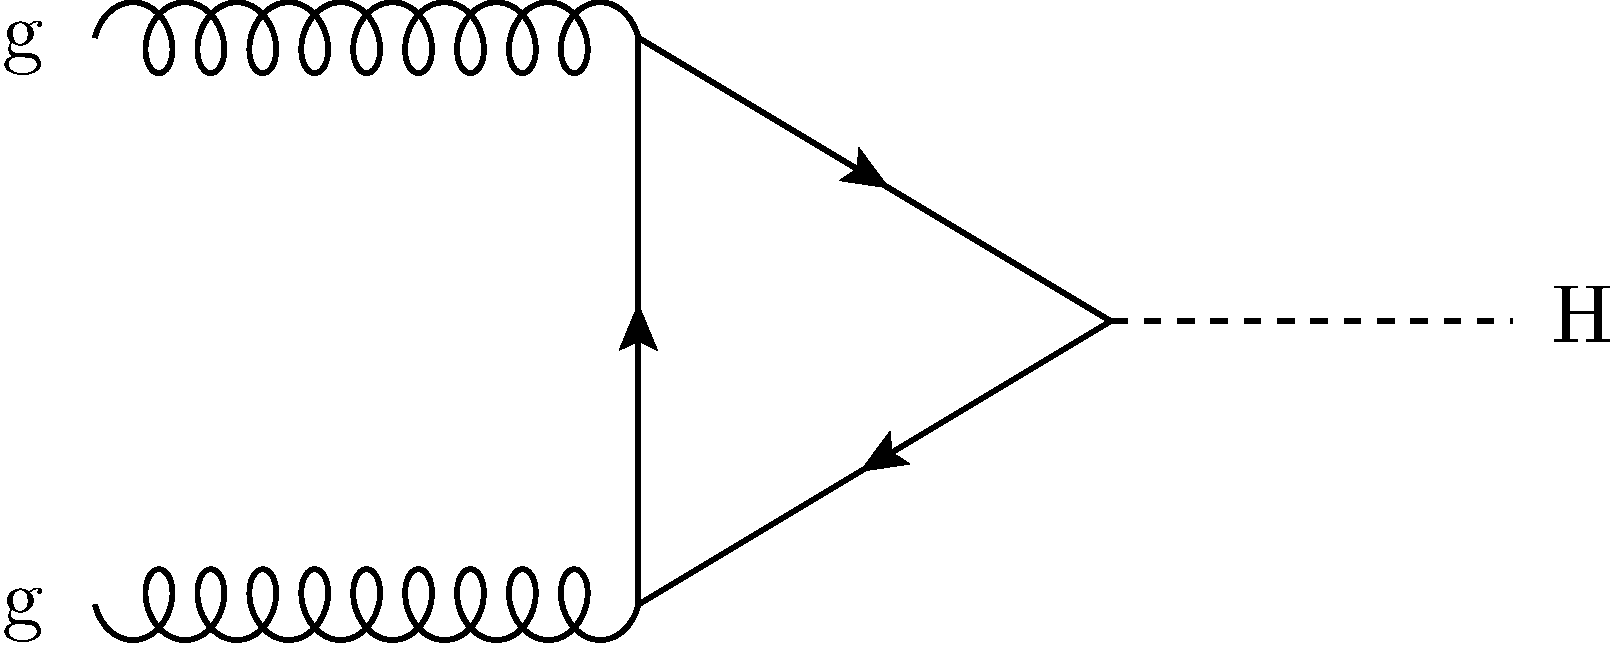
\includegraphics[width=0.45\textwidth]{Chapter01/Images/feynman_ggH.pdf}} \qquad
\subfloat[]{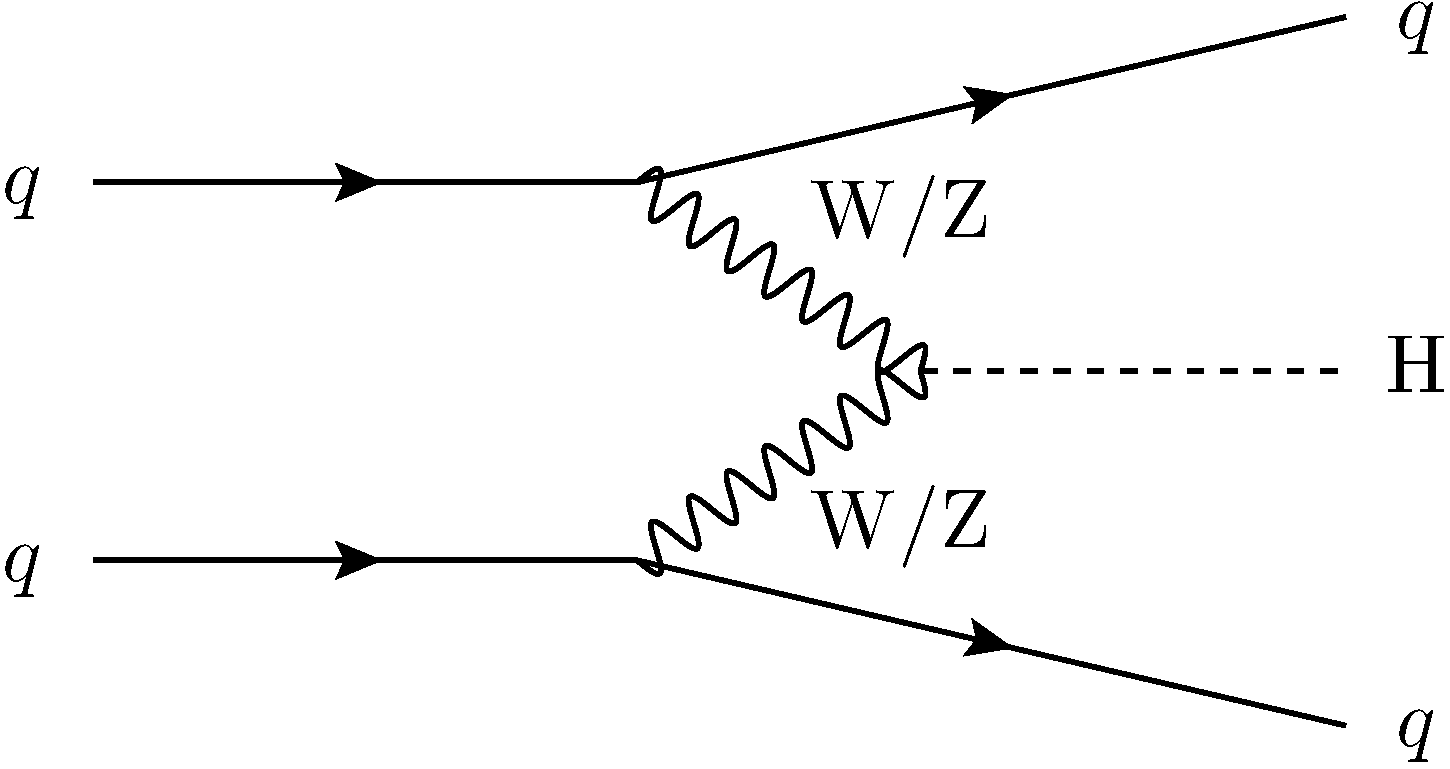
\includegraphics[width=0.45\textwidth]{Chapter01/Images/feynman_qqH.pdf}} \\
\subfloat[]{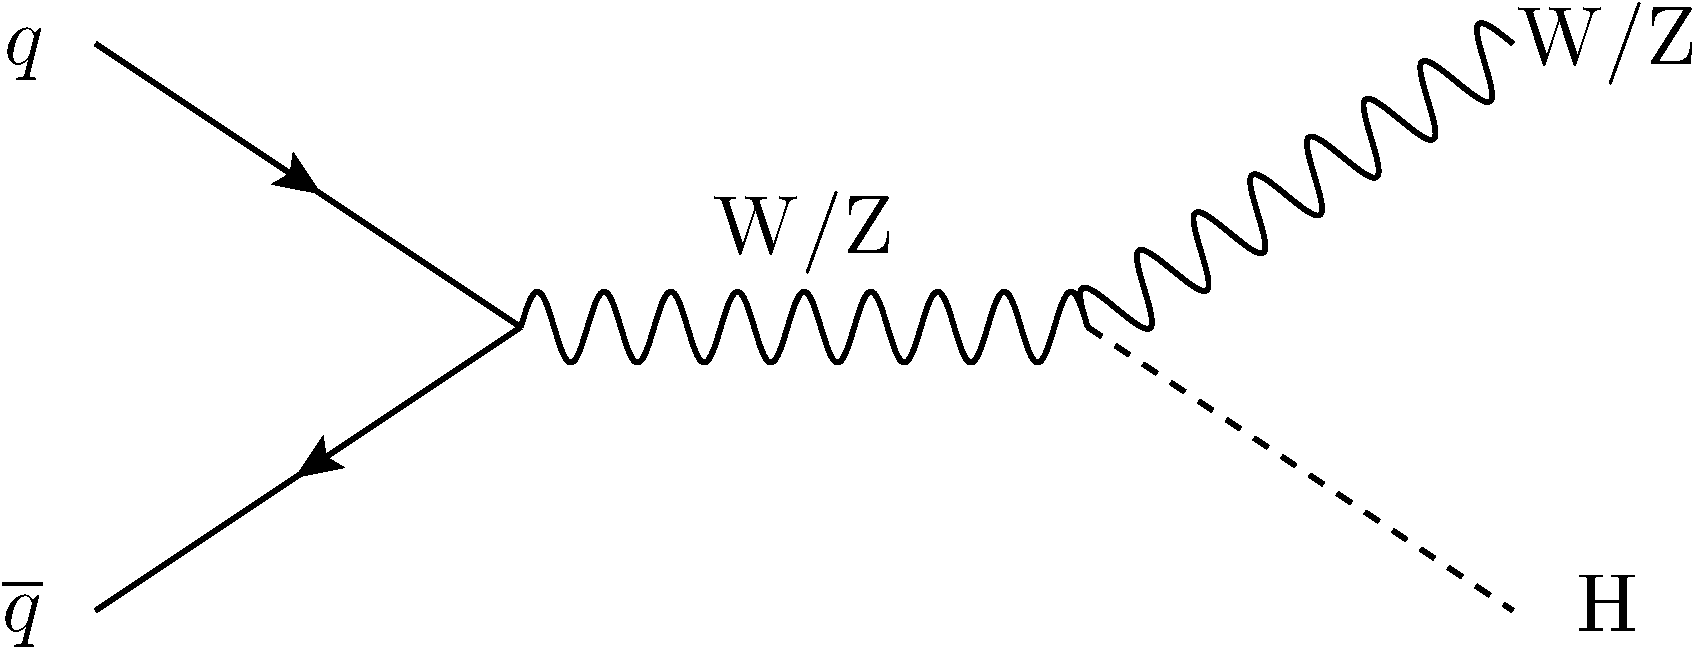
\includegraphics[width=0.45\textwidth]{Chapter01/Images/feynman_VH.pdf}}  \qquad
\subfloat[]{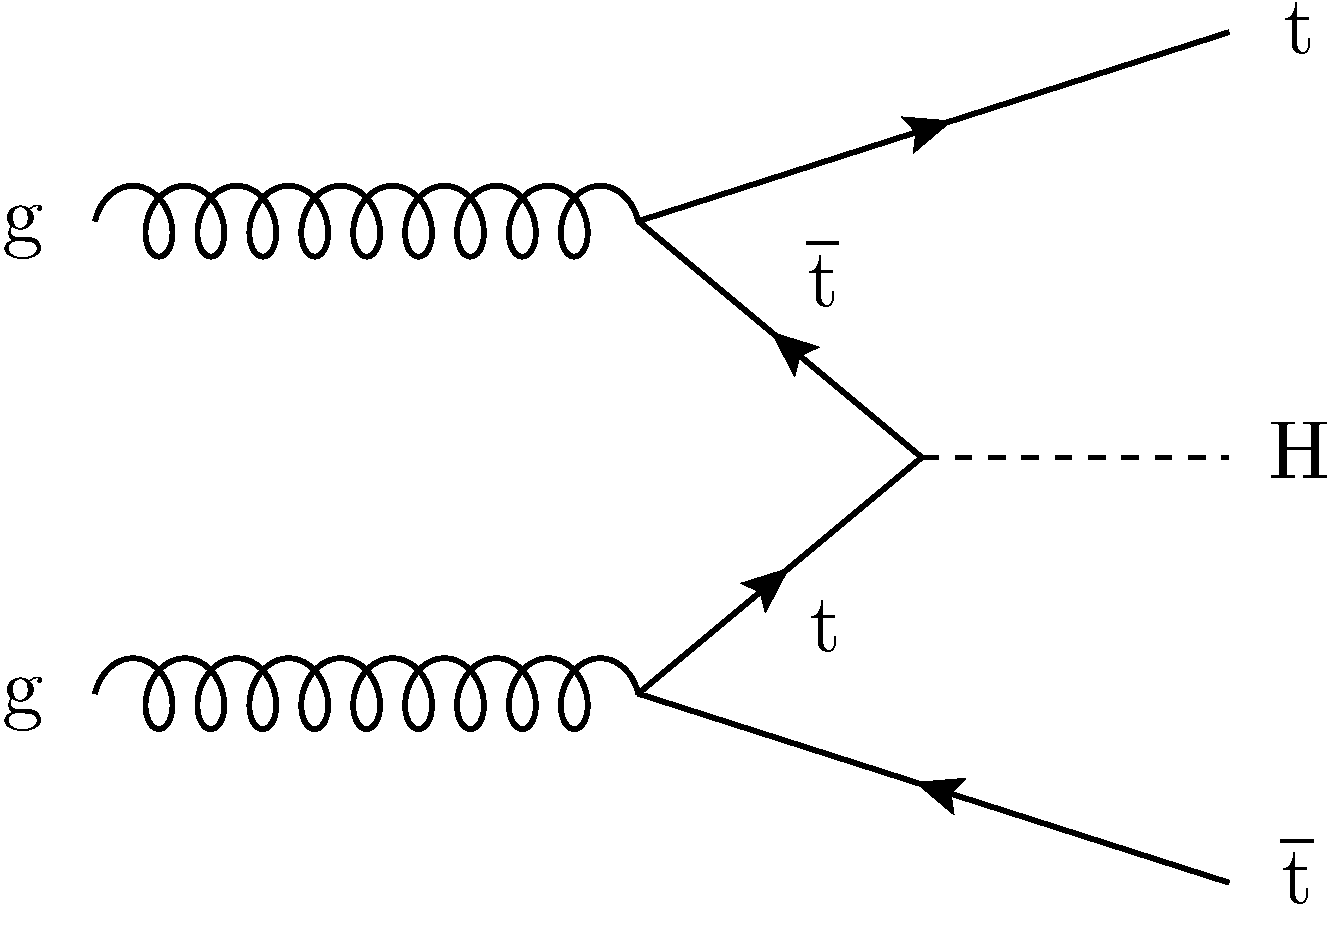
\includegraphics[width=0.45\textwidth]{Chapter01/Images/feynman_ttH.pdf}} \\
\caption[Feynman diagrams for the dominant production processes of the SM Higgs
boson.]{Feynman diagrams for the dominant production processes of the SM Higgs
boson. Shown is a) gluon fusion, b) vector boson fusion and
associated production with c) vector bosons and d) top quarks.}
\label{fig:SMFeynmanDiagrams}
\end{figure}

\begin{figure}[htbp]
 \includegraphics[width=0.7\textwidth]{Chapter01/Images/Higgs_XS_8TeV_lx.pdf}
\caption[Cross sections for Higgs production processes at $\sqrt{s}=8\,\TeV$ for
a range of Higgs boson masses.]{Cross sections for Higgs production processes at
$\sqrt{s}=8\,\TeV$ for a range of Higgs boson masses $m_{\PH}$~\cite{ARTICLE:HandbookofLHCHiggsCrossSectionsHiggsProperties}. Across the
mass range the gluon-fusion mode dominates, followed by the vector boson fusion
and associated production modes. The widths of the lines represent the
theoretical uncertainties on the cross section calculation.}
\label{fig:SMHiggsXS}
\end{figure}

\begin{figure}[htbp]
 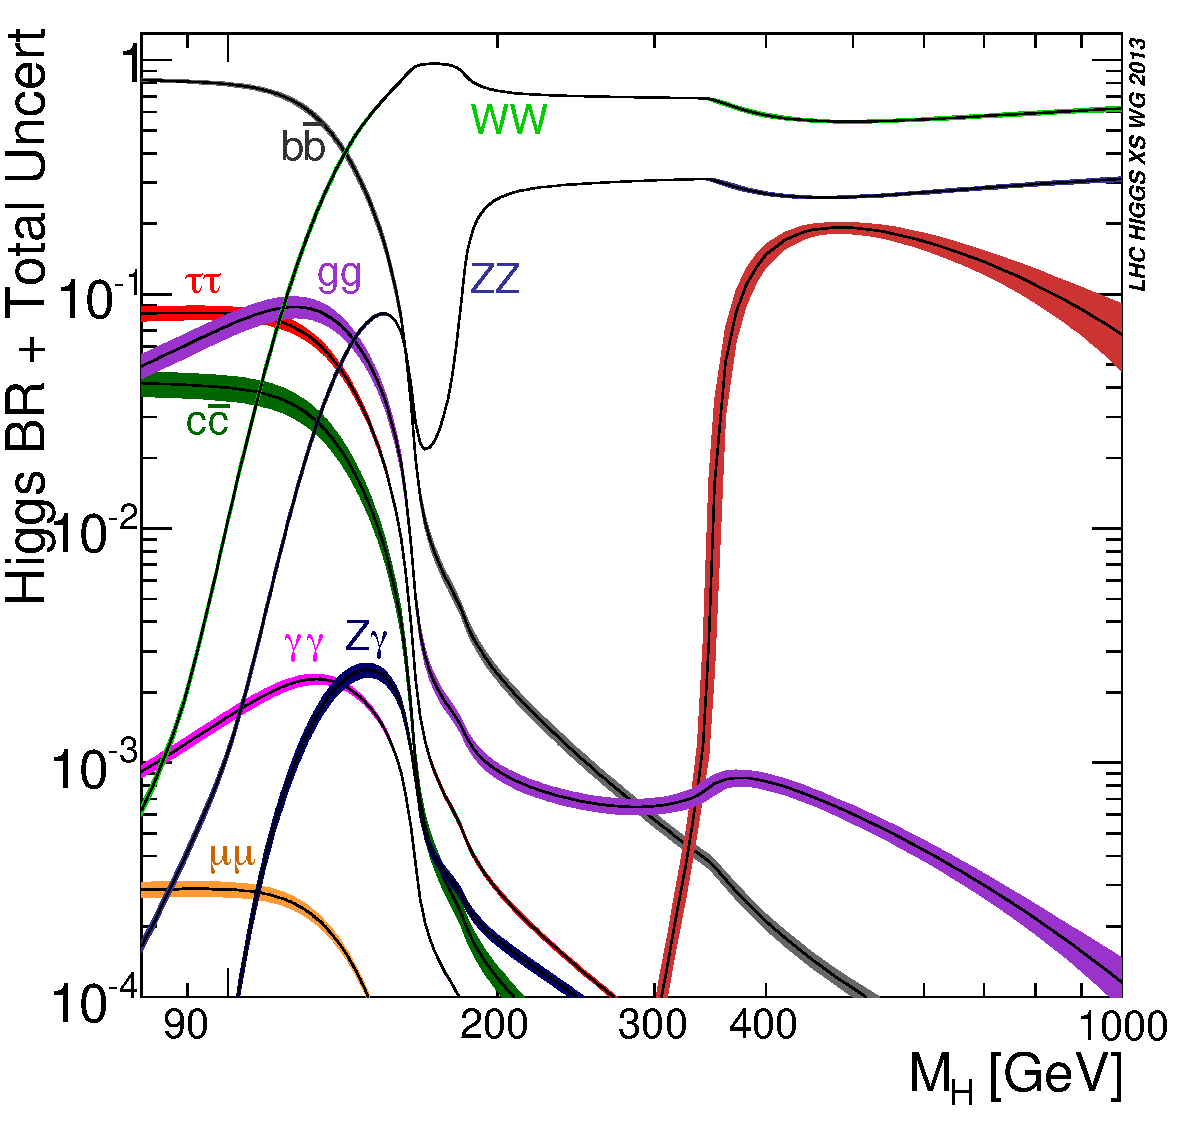
\includegraphics[width=0.6\textwidth]{Chapter01/Images/Higgs_BR.pdf}
\caption[Higgs boson branching ratios in the SM for a range of Higgs boson
masses.]{Higgs boson branching ratios in the SM for a range of Higgs boson
masses $m_{\PH}$ \cite{ARTICLE:HandbookofLHCHiggsCrossSectionsHiggsProperties}. At high masses, above their
kinematic thresholds, the $\PW\PW$,
$\PZ\PZ$ and $\ttbar$ (shown in red) decay modes dominate. 
At lower masses a wide range of different final states is possible. 
The widths of the lines represent the
theoretical uncertainties on the branching ratio calculation.}
\label{fig:SMHiggsBRs}
\end{figure}

% \subsection{Higgs Boson Production and Decay at the LHC}
% 
% At the LHC, protons are accelerated to higher energies than previously available at the 
% Tevatron. The increased centre-of-mass energy enhances the 
% rate at which Higgs boson production occurs and improves the sensitivity to higher 
% masses. The four main mechanisms by which a Higgs boson can be produced
% are shown at leading order in Figure~\ref{fig:higgsprodfeyn}.
% \begin{figure}[hbtp!]
% \begin{center}
% %\includegraphics[width=.49\textwidth]{theory/pheno/ggh.pdf}
% %\includegraphics[width=.49\textwidth]{theory/pheno/vh.pdf}\\
% %\includegraphics[width=.49\textwidth]{theory/pheno/qqh.pdf}
% %\includegraphics[width=.4\textwidth]{theory/pheno/tth.pdf}
% \includegraphics[width=\textwidth]{theory/pheno/allprods_new.pdf}
% \caption{Dominant SM Higgs boson production mechanisms: Gluon-gluon fusion (top left),
% vector-boson fusion (bottom left), associated production with vector boson (top right) 
% and top anti-top quark pair (bottom right).}
% \label{fig:higgsprodfeyn}
% \end{center}
% \end{figure}
% The dominant production mechanism is through gluon-gluon fusion ($ggH$). As the gluons
% are massless particles, the gluons couple to the Higgs boson via a quark-loop.
% The three other production mechanisms which dominate Higgs boson production are 
% vector boson fusion ($qqH$) and production in association with 
% a $W$ or $Z$ boson ($VH$) or top anti-top quark pair ($ttH$).
% Although these modes are at least an order of magnitude smaller in cross-section
% than gluon-gluon fusion, their specific topologies 
% can be exploited experimentally to enhance the signal over background processes 
% (see Chapter~\ref{chap:combinations}).
% Figure~\ref{fig:higgsprod} shows the production cross-sections and their theoretical 
% errors for the four main production modes of the SM Higgs boson in  
% p-p collisions at the LHC~\citep{lhcxswg2011,lhcxswg2012}.
% \begin{figure}[hbtp!]
% \begin{center}
% \includegraphics[width=0.8\textwidth]{theory/pheno/Higgs_XS_7TeV.pdf}\\
% \includegraphics[width=0.8\textwidth]{theory/pheno/Higgs_XS_8TeV_lx.pdf}
% \caption{SM Higgs boson production cross-sections at $\sqrt{s}=7~\mathrm{TeV}$ (top)
% and 8 TeV (bottom) of the four main production mechanisms, $pp\rightarrow H+X$,
% along with their theoretical uncertainties as a function of 
% $\mh$~\citep{lhcxswg2011,lhcxswg2012}. The coloured bands indicate the theoretical
% uncertainties.}
% \label{fig:higgsprod}
% \end{center}
% \end{figure}
% The Higgs boson is an unstable particle so will be observable directly at the LHC
% only through its decay products. The relative decay rates (branching ratios) to 
% different SM particles vary as a function of the Higgs boson mass.
% At low mass, $\mh<135$ GeV, Higgs boson decay to a $b$ anti-$b$ quark pair
% dominates. In proton-proton collisions, pairs of $b$-quarks are produced 
% frequently making the background levels too high to compete with for an experimental
% search. For higher masses, $\mh>180$ GeV, the Higgs boson is heavy enough
% to facilitate production of real $W$ and $Z$ bosons which dominate its decay.
% As the gluon and photon are massless, they do not directly couple to the Higgs boson
% hence these decays are mediated by virtual loops of massive particles.
% The branching ratios of the Higgs boson to SM particles are shown as a function
% of $\mh$ in Figure~\ref{fig:higgsdecay} (left).
% 
% For small $\mh$, the natural width of the SM Higgs boson, $\hwidth$, is several
% orders of magnitude smaller than its mass. Figure~\ref{fig:higgsdecay} (right) shows the 
% value of the SM Higgs boson total width as a function of its mass.
% This means that for decays in which the products are fully reconstructible in particle
% detectors, the width of the invariant mass spectrum of the decay products will depend almost entirely
% on the experimental resolution. 
% In particular the ATLAS and CMS detectors provide excellent energy and momentum resolution 
% for electrons, muons and photons.
% Despite having lower branching ratios,  the $\Hgg$ and $\Hzzl$ channels
% are therefore of particular importance for direct detection of the SM Higgs boson
% at the LHC.
% 
% 
% \begin{figure}[hbtp]
% \begin{center}
% \includegraphics[width=0.49\textwidth]{theory/pheno/YRHXS_BR_fig3.pdf}
% \includegraphics[width=0.49\textwidth]{theory/pheno/YRHXS_BR_fig2.pdf}
% \caption{Left: SM Higgs boson production branching ratios for 
% the dominant decays as a function of $\mh$. Right: SM Higgs boson total width, $\hwidth$, as 
% a function of $\mh$~\citep{lhcxswg2011}.}
% \label{fig:higgsdecay}
% \end{center}
% \end{figure}

\subsection{Higgs Invisible decays}

\colorbox{red}{
\begin{minipage}{0.95\linewidth}
TODO: 
\begin{itemize}
  \item Explain what are SM Higgs invisible decays.
  \item Go over the possibility of BSM invisible decays.
\end{itemize}

\end{minipage}
}

% Adding a bunch of references
\cite{ARTICLE:Higgs_SpontaneousSymmetryBreakdown}
\cite{BOOK:Griffiths}




















% 

% 

% 

